In video QoE assessment, perceptual factors \citep{Survey_QoE} including video quality, rebuffering frequency, rebuffering duration are directly perceived by the user.
Sub-section \ref{BiLSTM:subsec:InputFeatures} has introduced four input features (i.e. STSQ, PI, NR, and TR) that are related to perceptual factors.
These input features are fed into an LSTM-QoE model \citep{QoEModel_LSTM} to predict the instantaneous QoE as follows \citep{QoEModel_LSTM}:

\begin{equation}
    q(t) = LSTM^{0}(\bm{x}(t), \bm{c}(t-1))
\end{equation}
where, $q(t)$ represents the predicted instantaneous QoE at the time instant $t$, $\bm{x}(t)$ is the input features, $\bm{c}(t)$ is the memory cells which encode the knowledge of the inputs that have been observed up to the time $t$. $LSTM$ provides two functionalities: $LSTM^{0}$ for output QoE prediction and $LSTM^{c}$ for memory cells update which is given by  \citep{QoEModel_LSTM}:

\begin{equation}
    \bm{c}(t) = LSTM^{c}(\bm{c}(0:t-1), q(0:t-1)), \forall t \ge 1
\end{equation}

where, $\bm{c}(0:t-1)$ and $q(0:t-1)$ respectively refer to the past memory cells and the past predicted QoE.


The architecture of LSTM-QoE model are illustrated in Figure \ref{fig:LSTM}.

\begin{figure}[tb]
  \begin{center}
    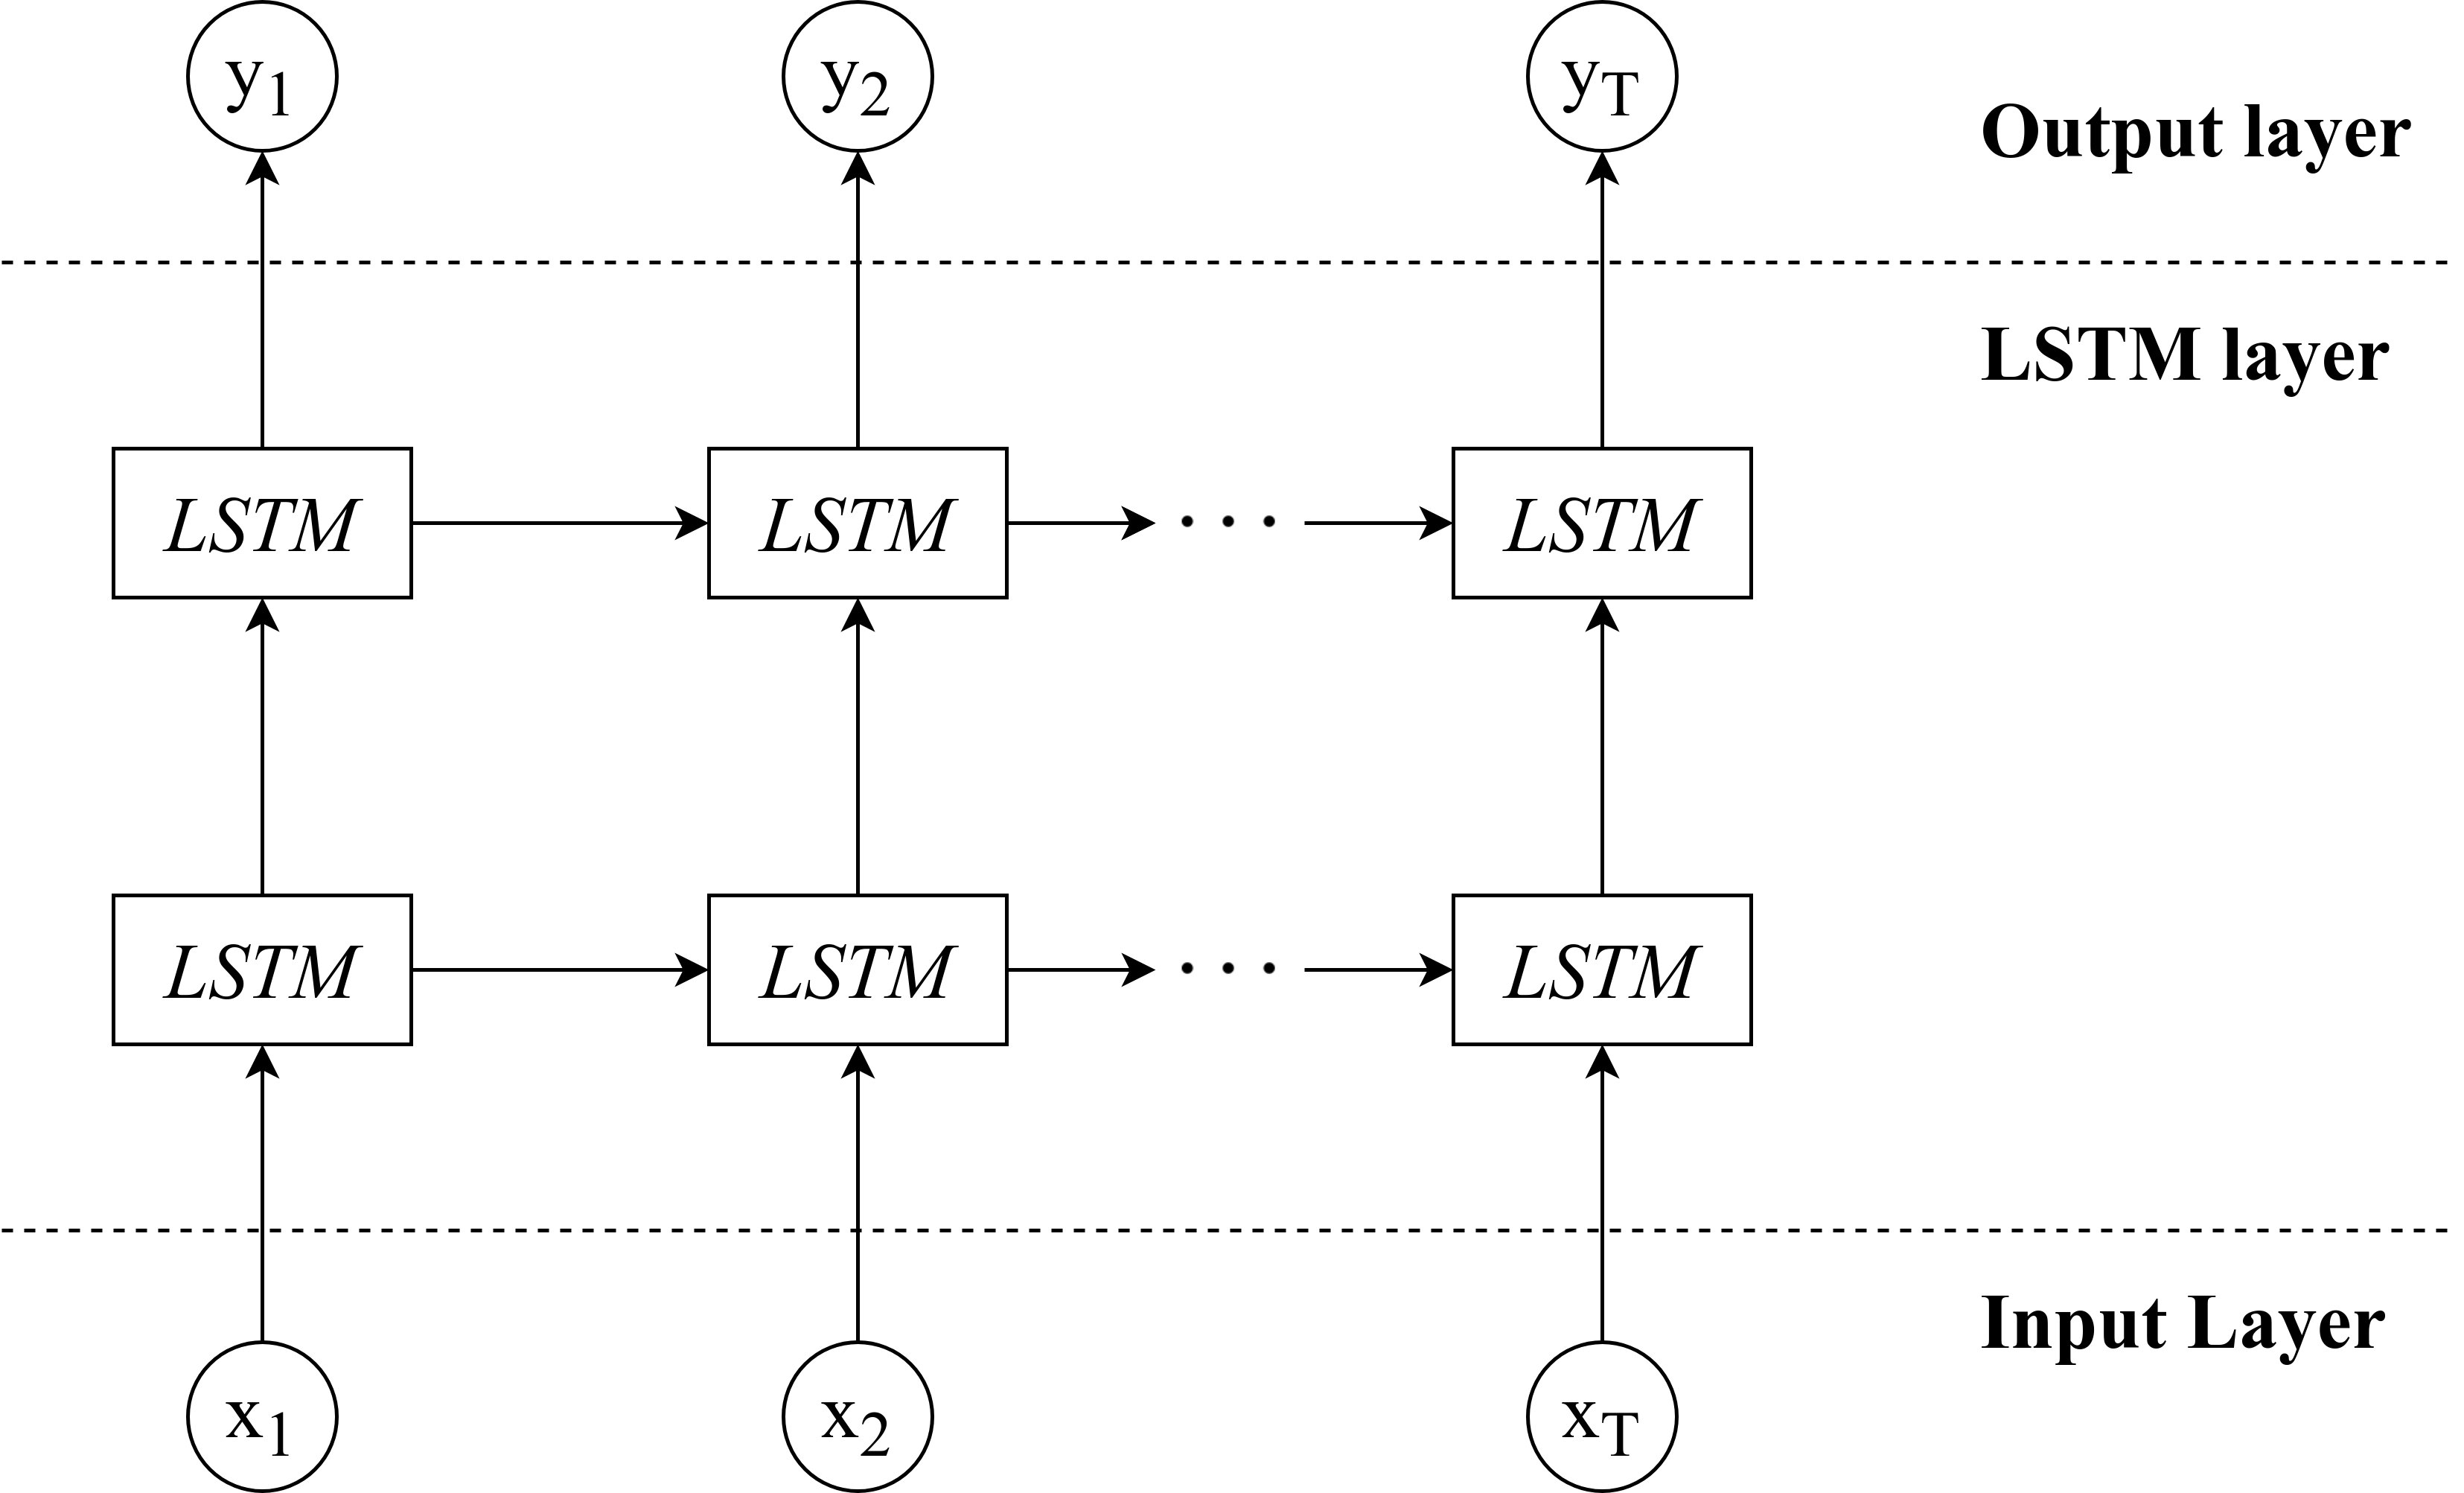
\includegraphics[width=0.6\linewidth]{\FigsDir/LSTM.png}
  \end{center}
  \caption{LSTM network \citep{QoEModel_LSTM} for the user's instantaneous QoE prediction. The network is composed of two LSTM (Long Short-term Memory) layers. The inputs to the layers are four features including STSQ, PI, NR, and TR. The outputs combine the LSTM layers' hidden states, representing the predicted instantaneous QoE values.}
  \label{fig:LSTM}
\end{figure}